\documentclass{article}

\include{stddefs}
\include{imodefs}

\chapterno{4}

\begin{document}

\chapter{What is optimization?}


In this chapter we will denote the set of column vectors with $d$ rows by $\RR^d$.
The arithmetic
of $d\times 1$ matrices apply i.e., we may add vectors in $\RR^d$ and
multiply them by a number in $\RR$.

In the next chapter we will introduce them as \emph{euclidean} vector spaces. The
term euclidean refers to a norm: a function measuring the size of a vector. In this
chapter we only need the structure as column vectors.


\section{What is an optimization problem?}

An optimization problem consists of maximizing or minimizing a function subject
to constraints.

Below are two classical examples related to minimizing (non-linear) functions subject to
(non-linear) constraints. These are actually examples of
convex optimization problems. More about that later.

\begin{example}

  A cylindrical can is supposed to have a volume of $V$ $\text{m}^3$. The material used
  for the top and bottom costs $T$ DKK per $\text{m}^2$ and the material used for
  the side costs $S$ DKK per $\text{m}^2$. Give the dimensions $r$ and $h$ of the
  can minimizing the prize of the materials.
  
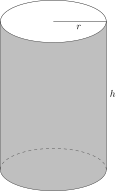
\includegraphics{cylinder.svg}

The cost of the top and bottom pieces are $2 \pi r^2 T$. The cost of the
side material is $2\pi r h S$. The constraint is that the volume must be
$V$. This is expressed in the equation $\pi r^2 h = V$. All in all
the optimization problem is
\begin{align*}
  &\text{Minimize} &2\pi r^2 T + 2\pi r h S&\\
  &\text{with constraints}\\
  &&\pi r^2 h &= V\\
  &&r &\geq 0\\
  &&h &\geq 0,
\end{align*}
where $V, T$ and $S$ are constants.

\end{example}

\begin{example}
  A person is in distress $D$ meters from the beach. The life guard
  spots the situation, but is $d$ meters from where he would naturally jump
  in the water as indicated below. The life guard runs $8$ m/s on the
  beach and swims $1$ m/s in the water. How far ($x$) should he run along the
  beach before jumping into the water in order to minimize the time needed
  to reach the person in distress?
  
  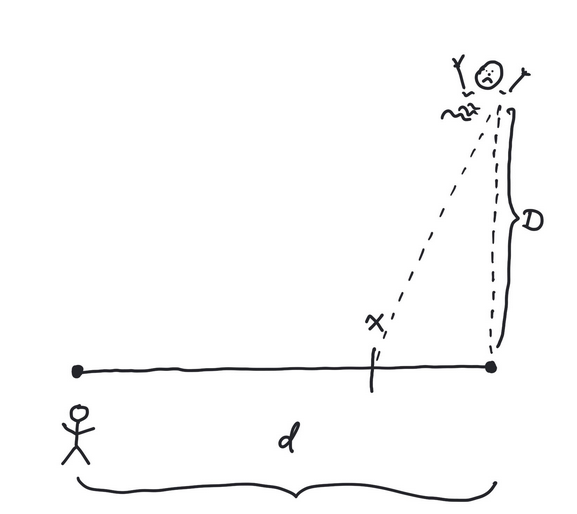
\includegraphics{lifeguard.png}

  The time spent moving with a speed of $v$ over a distance of $s$ is
  $$
  t = \frac{s}{v}.
  $$
  If the life guard jumps in the water at the point $x$ he will have
  to swim a distance of
  $$
  \sqrt{D^2 + (d-x)^2}
  $$
  using the Pythagorean theorem. Therefore the optimization problem becomes
\begin{align*}
  &\text{Minimize} &\frac{x}{8} + \sqrt{D^2 + (d-x)^2}&\\
  &\text{with constraints}\\
  &&x\geq 0\\
\end{align*}
Strictly speaking we do not need the constraint $x\geq 0$, as the life guard is free
to run in the other direction. So the optimization problem is simply to minimize
$$
\frac{x}{8} + \sqrt{D^2 + (d-x)^2}
$$
with no strings attached i.e., $x\in \RR$ is just assumed to be any number.


\begin{sage}
D = 200
d = 100
plot(x/8 + sqrt(D**2 + (d-x)**2), (x, 0, d))
\end{sage}

\end{example}


\beginshex
  You need to build a rectangular fence in front of your house for a herb garden.
  Your house will make up one side of the rectangle, so you only need to build three
  sides. Suppose you have 10 m of wire. What is the maximum area of the herb garden you can
  wall in?
\endshex


\section{General definition}

An optimization problem consists of a subset $D\subseteq \RR^d$ and
a function $f:D\rightarrow \RR$. We will consider optimization problems in the context
of minimization. Optimize in this situation means minimize.

\begin{definition}[emph]\label{defopt}
  In our most general setting an optimization problem looks like
\begin{align*}
  &\text{Minimize} &f(x)&\\
  &\text{with constraint}\\
  &&x\in C,
\end{align*}
     where $C$ and $D$ are subsets of $\RR^d$ with $C\subseteq D$ and $f: D\rightarrow \RR$ is a function.
A solution to the optimization problem is a vector $x_0\in C$, such that
$$
f(x_0) \leq f(x)
$$
for every $x\in C$. Here $x_0$ is called an \emph{optimum} and $f(x_0)$ is called the \emph{optimal value}.
\end{definition}

  The complexity of the problem depends very much on the nature of $C$ and $f$. Also,
  we cannot even be certain that an optimization problem has a solution. Consider
  the problem

  \begin{align*}
    &\text{Minimize} &x\\
    &\text{with constraint}\\
    &&x\leq 0
  \end{align*}

  Here $x$ can be made arbitrarily small subjsect to the constraint $x\leq 0$ and
  the problem has no solution.

  \beginshex
    How do you turn a maximization problem
\begin{align*}
  &\text{Maximize} &f(x)&\\
  &\text{with constraint}\\
  &&x\in C,
\end{align*}
    into a minimization problem?
    \endshex


    \beginshex\label{mothercopt}
    Suppose that $a > 0$. Solve the optimization problem
\begin{align*}
    &\text{Minimize} &a x^2 + b x + c\\
    &\text{with constraint}\\
    &&x\in \RR.
  \end{align*}
    
    \endshex

    \section{Convex optimization}

    Particularly well behaved optimization problems are the convex ones. These are optimization
    problems, where $C\subseteq \RR^d$ is a convex subset and $f:C\rightarrow \RR$ a
    convex function in Definition \ref{defopt}. To define these concepts we first introduce
    the notion of 
    a line in $\RR^d$.

    \begin{definition}[emph]\label{defline}
      A line $L\subseteq \RR^d$ is a subset of the form
      $$
      L = \{u + t v \mid t\in \RR\},
      $$
      where $u, v\in \RR^d$ with $v\neq 0$.
    \end{definition}

    \beginshex
    Show in Definition \ref{defline} that if $L$ is given by $u$ and $v$, then
    you might as well replace $v$ by $\alpha v$, where $\alpha\neq 0$.  It gives
    the same line.
    \endshex
    
\begin{figure}
  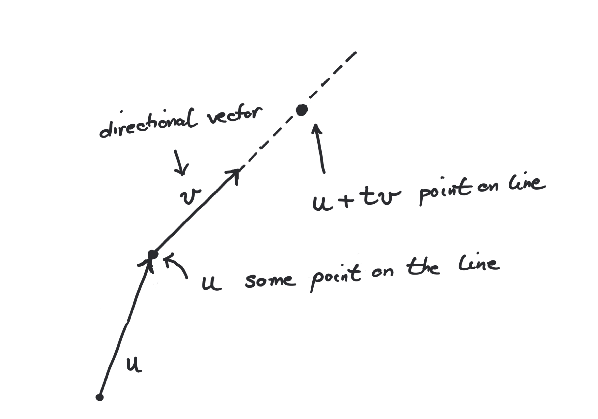
\includegraphics{line.png}
  \begin{center}
    Example of a line in $\RR^2$ with (directional) vector $v\in \RR^2$ through the point $u\in \RR^2$.
  \end{center}
\end{figure}


\begin{exercise}[emph]
  Show that there is a unique line passing through two distinct points
    $x, y\in \RR^d$ and that it is given by $u = x$ and $v = y - x$ in Definition \ref{defline}.
\end{exercise}

    \beginshex
    Do the points
    $$
    \begin{pmatrix}1\\ 2\\ 3\end{pmatrix}, \quad \begin{pmatrix} 4\\ 5\\ 6\end{pmatrix}
    \quad\text{and}\quad \begin{pmatrix} 7\\ 8\\ 9\end{pmatrix}
    $$
    lie on the same line in $\RR^3$?
    \endshex
    
    \beginshex
    Show that the line through two distinct points $x, y\in \RR^d$ is equal to the subset
    $$
    \{ (1-t) x + t y \mid t\in \RR\} \subseteq \RR^d.
    $$
    \endshex
    

    \begin{definition}[emph]
    A convex subset $C\subseteq \RR^d$ is a subset that contains the
    line segment between any two of its points $x, y\in C$ i.e.,
    $$
    (1 - t) x + t y\in C
    $$
    for every number $t$ with $0\leq t \leq 1$.
    \end{definition}

\begin{figure}
  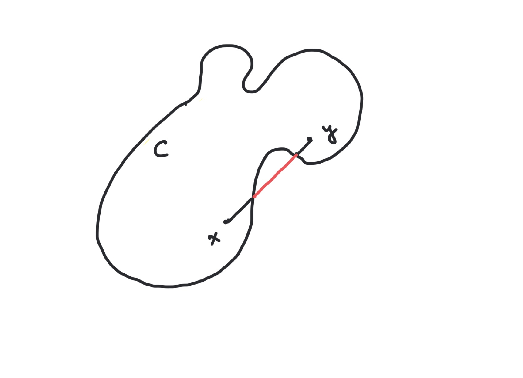
\includegraphics{nonconvex.png}
  \begin{center}
    Example of non-convex subset of $\RR^2$.
  \end{center}
\end{figure}


\begin{quizexercise}[showhide]
  \begin{quiz}
    \question
    Which of the subsets below are convex?
    \answer{T}
    $$C=\{1\}\subseteq \RR$$
    \answer{F}
    $$C=\{1, 2\}\subseteq \RR$$
    \answer{T}
    The points $C$ on a line $y = a x + b$ in $\RR^2$.
    \answer{F}
    $$
    C=\{(x, y)\in \RR^2 \mid x y \geq 0\}.
    $$
  \end{quiz}
\end{quizexercise}

    \beginshex
      A closed interval in $\RR$ is a subset of the form
      $$
      [a, b] = \{x \mid a \leq x \leq b\}
      $$
      for $a \leq b$. Prove that $[a, b]$ is a convex subset of $\RR$.
      \endshex

   % \beginshex
   % Give an example of a subset $S\subseteq \RR^2$ that is convex and one that is not convex.
   % \endshex

    \beginshex
    Let $A$ and $B$ be convex subsets of $\RR^d$. Prove that $A\cap B$ is a
    convex subset of $\RR^d$. Generalize this to show that if $A_1, \dots, A_n$
    are any number of convex subsets of $\RR^d$, then their intersection
    $$
    A_1 \cap \cdots \cap A_n
    $$
    is a convex subset of $\RR^d$. Is the union of two convex subsets necessarily convex?
    \endshex
    
    \begin{definition}[emph]
    A convex function is a function $f: C\rightarrow \RR$
    defined on a convex subset $C\subseteq \RR^d$, such that
    $$
    f((1 - t) x + t y) \leq (1-t) f(x) + t f(y)
    $$
    for every number $t$ with $0\leq t \leq 1$.
    \end{definition}

\begin{figure}
  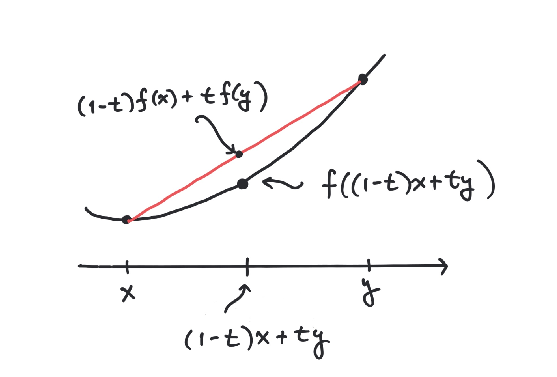
\includegraphics{convexfct.png}
  \begin{center}
    Graph of convex function. The line segment between $(x, f(x))$ and $(y, f(y))$
    lies above the graph.
  \end{center}
\end{figure}


    
    \beginshex
    Let the function $f: \RR \rightarrow \RR$ be given by
    $f(x) = a x + b$, where $a, b\in \RR$. Show that $f$ is a convex
    function.

    \begin{hideinbutton}{Hint}
      Try the case $a = 0$ first.
    \end{hideinbutton}

    Can you at this point prove that $f(x) = x^2$ is a convex function?

    \begin{hideinbutton}{Hint}
      Simplify
      $$
      (1 - t) x^2 + t y^2 - ((1-t) x + t y)^2
      $$
      to an expression that has to be non-negative.
      
      \begin{hideinbutton}{Hint}
        \begin{sage}
from sympy.abc import x, y, t
f = (1-t)*x^2 + t*y^2 - ((1-t)*x + t*y)^2
factor(f)
        \end{sage}
    \end{hideinbutton}
  \end{hideinbutton}

  Using that $f(x) = x^2$ is a a convex function, prove that $g(x) = x^4$ is a convex function and in general, that $h(x) = x^m$ is a convex function, where
  $m = 2n$ is an even natural number.

\begin{hideinbutton}{Hint}
      $$g(x) = f(x)^2$$
    \end{hideinbutton}
  
    It is a fact that $f(x) = x^3$ is not a convex function, but can
    you explain this using the definition of a convex function?

    \begin{hideinbutton}{Hint}
      Try $x = -1, y = 0$ and $t =\frac{1}{2}$.
    \end{hideinbutton}
    \endshex

    \begin{exercise}[emph]
    Let $f: \RR^d\rightarrow \RR$ be a convex function. Show that the subset
    $$
    C = \{x\in \RR^d \mid f(x) \leq a\}
    $$
    is a convex subset of $\RR^d$, where $a$ is a number.
    \end{exercise}
    

    We do not have the tools yet to prove the crucial
    result about convex optimization problems, but at least we can state it.


    \begin{remark}[emph]
    In hunting for optimal solutions to an optimization problem one is often stuck with a
    point $x_0\in \RR^d$, which is optimal locally. This means that $f(x_0)\leq f(x)$ for
    every $x$ that is sufficiently close to $x$ (we will explain what this means in the next
    chapter). The remarkable thing that happens in a convex optimization problem is
    that if $x_0$ is optimal locally, then it is a global optimum! It satisfies
    $f(x_0)\leq f(x)$ not only for $x$ close to $x_0$, but for every $x\in C$.
\end{remark}
    
    The optimization problem in Exercise \ref{mothercopt} is a very typical convex optimization
    problem.

    Below you see a plot of the function (press Compute)
    $$
    f(x) = x^3 + 2 x^2 + x + 1
    $$
    restricted
    to the interval $[-1.5, 0]$. You can see that it has a local minimum around $-0.3$ and
    also that this minimum is not a global minimum (certainly $f(-1.4)$ is smaller). So $f(x)$
    is not a convex function on this interval (but if you look at it more locally on the
    interval $[-0.6, 0]$ it is a convex function.
    
    \begin{sage}
      plot(x**3+2*x**2+x+1, (x, -1.5, 0))
    \end{sage}

    \beginshex
    Solve the optimization problem
    \begin{align*}
    &\text{Minimize} &x^3 + 2 x^2 + x + 1\\
    &\text{with constraint}\\
      &&x\in C
    \end{align*}
    for $C = [-0.6, 0]$ and $C = [-2, 0]$.
    \endshex
    
  \section{Linear optimization}

  The simplest convex optimization problems are the linear ones. Recall that a
  linear function $f: \RR^d\rightarrow \RR$ has the form
  $$
  f\begin{pmatrix} x_1 \\ \vdots \\ x_n \end{pmatrix} =
  c_1 x_1 + \cdots + c_n x_n
  $$
  for $c_1, \dots, c_n\in \RR$. Usually we write this with matrix notation as
  $$
  f(x) = c^T x,
  $$
  where
  $$
  c =
  \begin{pmatrix} c_1 \\ \vdots \\ c_n \end{pmatrix}\qquad \text{and} \qquad
  x = \begin{pmatrix} x_1 \\ \vdots \\ x_n \end{pmatrix}.
  $$

  \beginshex
  Show that a linear function is convex.
  \endshex
  
  A linear optimization problem is not about minimizing a linear function over
  an arbitrary convex subset. We choose the convex subset as an intersection of
  subsets of the form
  $$
  \{x\in \RR^d\mid a^T x \leq b\},
  $$
  where $a\in \RR^d$ is a non-zero vector and $b\in \RR$ a number i.e.,
  a linear optimization problem has the form
  \begin{align*}
    &\text{Minimize} &c^T x\\
    &\text{with constraint}\\
      &&x\in C,
  \end{align*}
  where
  \begin{align}\label{linsubs}
    C &= \{x\in \RR^d \mid a_1^T x \leq b_1, \dots, a_m^T x\leq b_m\}\\
    &= \{x\in \RR^d \mid a_1^T x \leq b_1\} \cap \cdots \cap \{x\in \RR^d \mid a_m^T x \leq b_m\}
  \end{align}
  and $c, a_1, \dots, a_m\in \RR^d$ and $b_1, \dots, b_m\in \RR$.

  \beginshex
  Use a selection of previous exercises to show that
  the subset $C$ defined in \eqref{linsubs} is a convex subset of $\RR^d$.
  \endshex
  
  Using matrix notation we write $C$ as
  $$
  C = \{x\in \RR^d \mid A x \leq b\},
  $$
  where $A$ is the $m\times d$ matrix with row vectors $a_1^T, \dots, a_m^T$ and
  $$
  b =
  \begin{pmatrix}
    b_1 \\ \vdots \\ b_m
  \end{pmatrix}.
  $$

  \begin{example}\label{exlinopt}
  
     Here is a concrete example for $d = 2$. The optimization problem
  \begin{align*}
    &\text{Maximize} &x + y&\\
    &\text{with constraints}\\
    &&2 x + y &\leq 1\\
    &&x + 2 y &\leq 1\\
    &&x &\geq 0\\
    &&y &\geq 0
  \end{align*}
  translates into matrix notation with the matrices
  \newcommand{\mi}{\hphantom{-}}
  $$
  c = \begin{pmatrix} 1 \\ 1 \end{pmatrix}, \qquad
  A = \begin{pmatrix} \mi 2 & \mi 1 \\ \mi 1 & \mi 2 \\ -1 & \mi 0 \\ \mi 0 & - 1\end{pmatrix}\qquad \text{and}\qquad
  b = \begin{pmatrix} 1 \\ 1 \\ 0 \\ 0 \end{pmatrix}.
  $$

  In this case it is helpful to draw the optimization problem in the plane $\RR^2$. This is done below.
  
  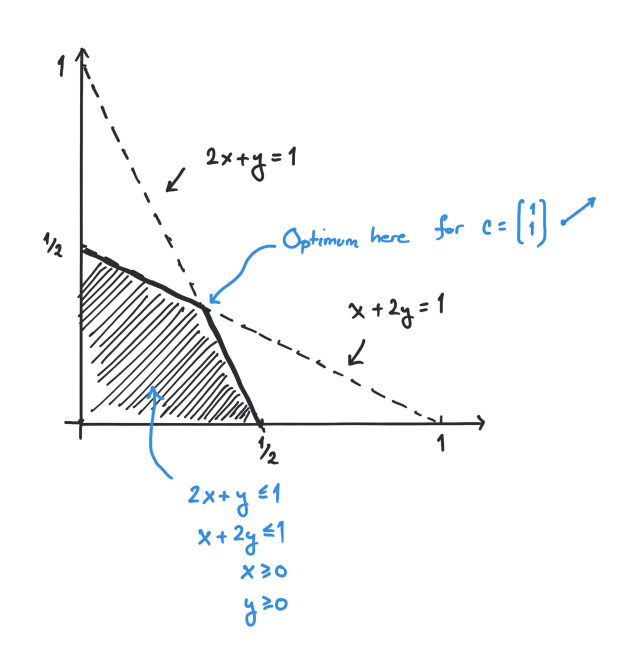
\includegraphics{LP.png}
  \begin{center}
    Constraints pictured as shaded area above. Optimum occurs in a vertex (corner).
    \end{center}
  
  \end{example}
  


  
  We will give a general (but rather slow) algorithm below for solving
  linear optimization problems. In fact it all boils down to solving
  systems of linear inequalities. Sometimes linear optimization is
  referred to as \url{linear
    programming}{https://en.wikipedia.org/wiki/Linear_programming}. The
  basic theory of linear programming was pioneered, among others, by
  one of the inventors of the modern computer, John von Neumann.

  
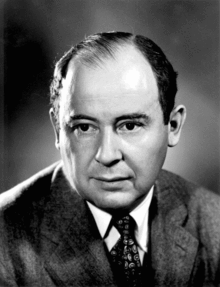
\includegraphics{vonNeumann.gif}
\begin{center}
  \url{John von Neumann}{https://en.wikipedia.org/wiki/John_von_Neumann} (1903-1957). Picture from \url{LANL}{https://en.wikipedia.org/wiki/Los_Alamos_National_Laboratory}.
\end{center}

  Sage has much more advanced algorithms built in for solving (integer) linear optimization
  problems. I have translated the linear optimization problem in Example \ref{exlinopt} into
  Sage below.

\begin{sage}
LP = MixedIntegerLinearProgram(solver = "GLPK")
 
# generate variables (do not require integer solution) 
x = LP.new_variable(integer=False)
 
# Linear function to be maximized (notice maximized!)

LP.set_objective(x[1] + x[2])
    
# Add constraints
LP.add_constraint( 2*x[1] + x[2] <= 1 );
LP.add_constraint( x[1] + 2*x[2] <= 1 );
LP.add_constraint( x[1] >= 0 );
LP.add_constraint( x[2] >= 0 );

 
LP.show()
 
oval = LP.solve()
xopt = LP.get_values(x);
 
print('Optimal Value:', oval)
print('occurs in')
for i, v in xopt.items():
    print('x_%s = %f' % (i, v))
\end{sage}
  
\section{Fourier-Motzkin elimination}

Fourier-Motzkin elimination is a classical method (dating back to 1826) for solving linear inequalities. 
It is also a key ingredient in an algorithm for solving linear optimization problems.

I am convinced that
the best way to explain this method is by way of an extended example. For more formalities you may
consult \url{Chapter 1}{https://www.worldscientific.com/doi/suppl/10.1142/8527/suppl_file/8527_chap01.pdf} of my book \url{Undergraduate Convexity}{https://www.worldscientific.com/worldscibooks/10.1142/8527}.

Consider the linear optimization problem

\begin{equation}\label{optfmex}
  \begin{array}{llrrrr}
    &\text{Maximize} &x + y\\
    &\text{with constraints}\\
    &&2 x &+ &y &\leq &6\\
    &&x &+ &2 y &\leq &6\\
    &&x &+ &2 y &\geq &2\\
    &&x && &\geq &0\\
    &&&&y &\geq &0.
  \end{array}
\end{equation}
  
We might as well write this as

$$
  \begin{array}{llrrrl}
    &\text{Maximize} &z\\
    &\text{with constraints}\\
    &&&& z &= &x + y\\
    &&2 x &+ &y &\leq &6\\
    &&x &+ &2 y &\leq &6\\
    &&x &+ &2 y &\geq &2\\
    &&x &&&\geq &0\\
    &&&&y &\geq &0
  \end{array}
$$
  
  by adding the extra variable $z$. This enables us to reformulate the problem as follows: Find
  the maximal value of $z$, such that there exists $(x, y)\in \RR^2$ with
  $$
  (x, y, z)\in P,
  $$
  where $P\subseteq \RR^3$ is the set of solutions to the system


\begin{equation}\label{Pset}

  \begin{array}{llrrrl}
    &&&& z &= &x + y\\
    &&2 x &+ &y &\leq &6\\
    &&x &+ &2 y &\leq &6\\
    &&x &+ &2 y &\geq &2\\
    &&x &&&\geq &0\\
    &&&&y &\geq &0
  \end{array}

\end{equation}
  
% \begin{align}\label{Pset}
%     && z&= x + 3 y\\
%     &&2 x + y &\leq 1\\
%     &&x + 2 y &\leq 1\\
%     &&x &\geq 0\\
%     &&y &\geq 0.
% \end{align}


  of \footnote{inequalities}{An equality $a = b$ is logically equivalent to the two
    inequalities $a\leq b$ and $a \geq b$ in the sense that $(a\leq b) \wedge (a\geq b) \iff a = b$.}.

  We have the Gauss elimination method for solving systems of linear equations. How do we now solve
  \eqref{Pset}, where we also have inequalities?

  Well, at first we can actually do a Gauss elimination step by eliminating $x$ in the equation
  $z = x + y$ i.e., by putting $x = z - y$. This is then inserted into the inequalities in
  \eqref{Pset}:

$$
\begin{array}{llrrrl}
    &&2 (z - y) &+ &y &\leq &6\\
    &&(z - y) &+ &2 y &\leq &6\\
    &&(z - y) &+ &2 y &\geq &2\\
    &&(z - y) &  &    &\geq &0\\
    &&          &  &  y &\geq &0
\end{array}
$$

and we get the system 

$$
  \begin{array}{llrrrl}
    &&2 z &- &y&\leq &6\\
    &&z &+ &y &\leq &6\\
    &&z &+ & y &\geq &2\\
    &&z &- &y &\geq &0\\
    &&  &  &y   &\geq &0
  \end{array}
$$
  of inequalities
  in the variables $z$ and $y$. Now we only have inequalities left and we have to invent a trick for
  eliminating $y$. Let us isolate $y$ on one side of the inequality signs $\leq$ and $\geq$:

  $$
    \begin{array}{llrrrl}
    &&2 z &- &6 &\leq &y\\
    &&6 &- &z &\geq &y\\
    &&2 &- &z &\leq &y\\
    && & &z &\geq &y\\
    &&&&0 &\leq &y
  \end{array}
$$
  
  Written a little differently this is the same as

\begin{equation}\label{fmex}
  \begin{array}{llrrrl}
    &&2 z &- &6&\leq &{\color{red} y} \\
    &&&&&&{\color{red} y} &\leq &6 &- &z\\
    &&2&- &z&\leq &{\color{red} y} \\
    &&&&&&{\color{red} y} &\leq &z\\
    &&&&0&\leq &{\color{red} y}
  \end{array}
\end{equation}

Now the scene is set for elimination of $y$. Listen carefully. First the inequalities in 
\eqref{fmex} can be boiled down to the following two inequalities

\begin{equation}\label{fmex1}
  \begin{array}{lllll}
\max(2 z - 6, 2 - z, 0) &\leq &{\color{red} y}\\
&& {\color{red} y} & \leq &\min(6 - z, z).
  \end{array}
\end{equation}
using (repeatedly) that  $\max(a, b) \leq c \iff a\leq c \wedge b\leq c$ and
  $c\leq \min(a, b) \iff c\leq a \wedge c\leq b$ for three
numbers $a, b, c\in \RR$.

Then, finally comes the (Fourier-Motzkin) elimination step: The existence of a solution to \eqref{fmex1} is
equivalent to the single inequality

\begin{equation}\label{singleineq}
\max(2 z - 6, 2 - z, 0) \leq \min(6 - z, z).
\end{equation}

This single inequality can be exploded or expanded (see Exercise \ref{explex}) into the following $6 = 3\cdot 2$ inequalities

\begin{align*}
2 z - 6 &\leq 6 - z\\
2 z - 6 &\leq z\\
2 - z &\leq 6 - z\\
2 - z &\leq z\\
0 &\leq 6 - z\\
0 &\leq z.
\end{align*}

Similarly to \eqref{fmex} we now isolate $z$ from the above inequalities:

\begin{equation*}
  \begin{array}{lllll}
&&&{\color{red} z} &\leq &4\\
&&&{\color{red} z} &\leq &6\\
&1&\leq &{\color{red} z}\\
&&&{\color{red} z} &\leq &6\\
&0&\leq &{\color{red} z}
\end{array}
\end{equation*}

and find that

\begin{equation*}
  \begin{array}{lllll}
\max(1, 0) = 1 &\leq &{\color{red} z}\\
&& {\color{red} z} & \leq &\min(4, 6) = 4.
  \end{array}
\end{equation*}


Therefore the maximum in the optimization problem \eqref{optfmex} is $z = x + y = 4$. 
How do we now find numbers $x, y\in \RR$ satisfying the constraints
in the optimization problem \eqref{optfmex} with $z = x + y = 4$?

This is simply done inserting first $z = 4$ in \eqref{fmex1}. Here you get the two inequalities
$2 \leq y$ and $y\leq 2$. Therefore $y = 2$. Since we had $x = z - y$ from the bery beginning
we therefore get $x = 2$ and we have the unique solution to the optimization problem.

\beginshex
What is the solution if we replace Maximize with Minimize in the optimization problem \eqref{optfmex}?
\endshex

  

\beginshex\label{explex}

Prove the following:

    Let $x_1, \dots, x_m, y_1, \dots, y_n\in \RR$ be $m + n$ numbers. Then
    $$
    \max(x_1, \dots, x_m) \leq \min(y_1, \dots, y_n)
    $$
    if and only if the $m n$ inequalities
    $$
    \begin{matrix}
      &x_1 \leq y_1 &x_1 \leq y_2 &\dots &x_1\leq y_n\\
      \\
      &\vdots & \vdots &\ddots &\vdots\\
      \\
      &x_m \leq y_1 &x_m \leq y_2 &\dots &x_m\leq y_n
    \end{matrix}
    $$
    are satisfied.
\endshex

\beginshex

The following is Exercise 1.8 from my book \url{Undergraduate Convexity}{https://www.worldscientific.com/worldscibooks/10.1142/8527}.

A vitamin pill $P$ is produced using two ingredients $M_1$
  and $M_2$. The pill needs to satisfy four constraints for the vital
  vitamins $V_1$ and $V_2$. It must contain at least $6$ milligrams and
  at most $15$ milligrams of $V_1$ and at least $5$ milligrams and at
  most $12$ milligrams of $V_2$. The ingredient $M_1$ contains $3$
  milligrams of $V_1$ and $2$ milligrams of $V_2$ per gram.  The
  ingredient $M_2$ contains $2$ milligrams of $V_1$ and $3$ milligrams
  of $V_2$ per gram:

$$
\def\arraystretch{1.5}
\begin{array}{c|cc}
& V_1 & V_2\\ \hline
M_1 & 3 & 2\\
M_2 & 2 & 3
\end{array}
$$


Let $x$ denote the amount of $M_1$ and $y$ the amount of $M_2$
  (measured in grams) in the production of a vitamin pill. Write down
  a system of linear inequalities in $x$ and $y$ describing the
  constraints above.

  We want a vitamin pill of minimal weight satisfying the
  constraints. How many grams of $M_1$ and $M_2$ should we mix?
  Describe how Fourier-Motzkin elimination can be used in solving this
  problem.





\endshex

  
\section{Application in machine learning and data science}


To start with, consider a toy example of a machine learning problem: we wish
to tell the gender of a person based on a data point consisting of
the height and weight of the person.

To do this we train our model by measuring the height and weight of a
lot of people. Each of these measured data points are labeled
female or male according to the gender of the person.

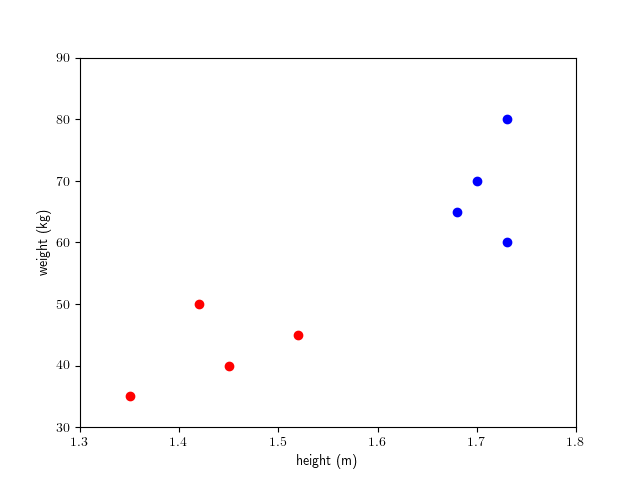
\includegraphics{sephp.png}

Given a new data point, we wish to tell if the person is female or male. Here we
consider a very simple model for doing this. First we need to introduce some
new mathematical terms. We will introduce the terms generally for
data points in $\RR^d$ and not just in $\RR^2$ as above.


A hyperplane in $\RR^d$ is a generalization of a line $y = a x + b$ in the plane. In general
a hyperplane is defined as the set of points $x\in \RR^d$ satisfying
$$
a^T x = b,
$$
where $a\in \RR^d$ is a non-zero vector and $b$ is a number. A hyperplane divides $\RR^d$
into two subsets: the points above or on the hyperplane satisfying $a^T x \geq b$ and the ones
below the hyperplane satisfying $a^T x < b$.


Suppose we are given a data set as a finite set of points in $\RR^d$ and that each of
these points are labeled with either a blue or a red color. We wish to
find a hyperplane, such that the blue points are above and the red points
are below the hyperplane.

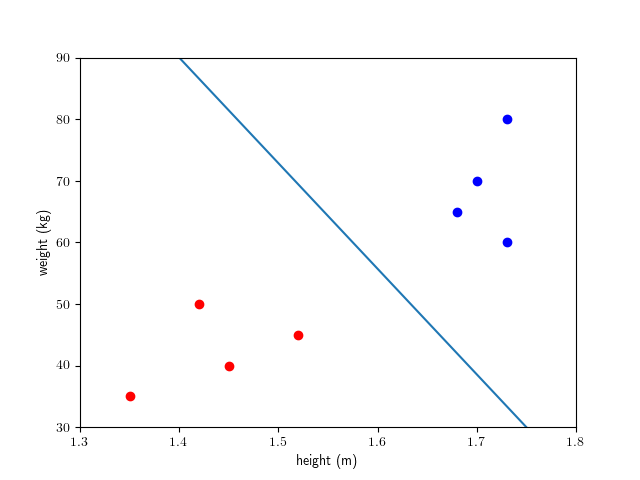
\includegraphics{sephpWithline.png}


We may then use the hyperplane to predict the label of a point. This could be
gender, if you win or lose money buying a stock, anything with
a binary classifier.



  
  \subsection{Formulation as a linear optimization problem}

  Suppose that the points labeled blue are $x_1, \dots, x_m\in \RR^d$ and
  the points labeled red are $y_1, \dots, y_n\in \RR^d$. Then we wish to
  find $a\in \RR^d$ and $b\in \RR$, such that
  $$
  a^T x_i > b
  $$
  for $i = 1, \dots, m$ and
  $$
  a^T y_j < b
  $$
  for $j = 1, \dots, n$. One can show that these strict inequalities may be solved 
  for $a$ and $b$ if and only if the inequalities
  \begin{align*}
  a^T x_i &\geq b + 1\\
  a^T y_j &\leq b - 1
  \end{align*}
  are solvable for $a$ and $b$, where $i = 1, \dots, m$ and $j = 1, \dots, n$.
  
  It is, however, not realistic to expect data to behave this nicely. Instead one invents
  the rather ingenious linear optimization problem

  \begin{align}\label{linoptnice}
    &\text{Minimize} &\frac{1}{m}(u_1 + \cdots + u_m) + \frac{1}{n}(v_1 + \cdots + v_n)\\
    &\text{with constraints}\\
    &&a^T x_i + u_i&\geq b + 1\\
    &&a^T y_j - v_j &\leq b - 1\\
    &&u_i&\geq 0\\
    &&v_j&\geq 0
  \end{align}
  
  for $i = 1, \dots, m$ and $j = 1, \dots, n$. This linear optimization problem has optimal value zero
  if and only if data can be separated strictly. Otherwise, it finds a hyperplane minimizing the mean errors
  for the points involved.

  The linear optimization problem \eqref{linoptnice} may look untied to the real world, but it has
  been used very successfully in the diagnosis and prognosis of breast
  cancer. See \url{Mangasarian et al.}{https://www.jstor.org/stable/171686}

  In the sage window below we have implemented the solution of the
  linear optimization problem \eqref{linoptnice}, where the output is
  a graphical illustration of the optimal line, that separates the
  points in \texttt{xpts} and \texttt{ypts} with the smallest mean
  error as defined in the function to be minimized in \eqref{linoptnice}.
  
\begin{sage}
# Enter blue data points below
xpts = [(3, 1), (4, 2), (4, 3), (3, 5)]
# Enter red data points below
ypts = [(2, 2), (2.5, 4.5), (3, 2), (4, 1)]

LP = MixedIntegerLinearProgram(solver = "GLPK", maximization=False)
 
# generate variables (do not require integer solution) 
a = LP.new_variable(integer=False)
b = LP.new_variable(integer=False)
u = LP.new_variable(integer=False, nonnegative=True)
v = LP.new_variable(integer=False, nonnegative=True)



# Linear function to be minimized

LP.set_objective(float(1)/len(xpts)*sum(u[i] for i in range(1, len(xpts)+1)) + float(1)/len(ypts)*sum(v[i] for i in range(1, len(ypts)+1)))
    
# Add constraints

for i in range(1, len(xpts)+1):
  LP.add_constraint(xpts[i-1][0]*a[1] + xpts[i-1][1]*a[2] + u[i] >= b[1] + 1)

for j in range(1, len(ypts)+1):
  LP.add_constraint(ypts[j-1][0]*a[1] + ypts[j-1][1]*a[2] - v[j] <= b[1] - 1)
 
# LP.show()
 
oval = LP.solve()
aopt = LP.get_values(a);
bopt = LP.get_values(b)

# Compute frame for showing separating line

pts = xpts + ypts
xvals = list(map(lambda x: x[0], pts))
yvals = list(map(lambda y: y[1], pts))

xmin = min(xvals)
xmax = max(xvals)
ymin = min(yvals)
ymax = max(yvals)


# Intersection of separating line with frame (cumbersome!):

if (aopt[2] == 0):
  x =  bopt[1]/aopt[1]
  p1 = (x, ymin)
  p2 = (x, ymax)
else:
  a = -aopt[1]/aopt[2]
  b = bopt[1]/aopt[2]
  y = a*xmin + b
  if (y >= ymin and y <= ymax):
    p1 = (xmin, y)
    x = (ymax - b)/a
    if (x > xmin and x <= xmax):
      p2 = (x, ymax)
    else:
      x = (ymin - b)/a  
      if (x >= xmin and x <= xmax):
        p2 = (x, ymin)
      else:
        p2 = (xmax, a*xmax+b)
  else:
    x = (ymax - b)/a
    if (x >= xmin and x <= xmax):
      p1 = (x, ymax)
      y = a*xmax + b
      if (y >= ymin and y < ymax):
        p2 = (xmax, y)
      else:
        x = (ymin -b)/a
        p2 = (x, ymin)
    else:
      p1 = (xmax, a*xmax + b)
      x = (ymin - b)/a
      p2 = (x, ymin)
      
show(points(xpts, rgbcolor=(0, 0, 1), pointsize=30) + points(ypts, rgbcolor=(1,0,0), pointsize=30) + line([p1, p2], rgbcolor=(100, 100, 100), linestyle='dashed')) 
\end{sage}


\end{document}











